% 基尔霍夫电路定律

\pentry{电路\upref{Circ}}

\begin{theorem}{基尔霍夫电流定律}
\textbf{基尔霍夫电流定律}又称为\textbf{基尔霍夫第一定律},规定在电路中所有进入某节点的电流的总和等于所有离开这节点的电流的总和. 或者说,假设进入某节点的电流为正值,离开这节点的电流为负值,则所有涉及这节点的电流的代数和等于零.以方程式表达,对于电路的任意节点,有
\begin{equation}
\sum_{k=1}^n i_k =0
\end{equation}
其中,$i_k$是第$k$个进入或离开这节点的电流,是流过与这节点相连接的第$k$个支路的电流,可以是实数或复数.
\end{theorem}

\subsubsection{证明}
考虑电路的某节点,跟这节点相连接有$n$个支路.假设进入这节点的电流为正值,离开这节点的电流为负值,则这节点的总电流$i$等于流过支路$k$的电流$i_k$的代数和:
\begin{equation}
i=\sum_{k=1}^n i_k
\end{equation}
将这方程式对某段时间 $[t_1, t_2]$ 内积分,可以得到这段时间该节点电荷的增加
\begin{equation}
q=\sum_{k=1}^n q_k
\end{equation}
其中 $q = \int_{t_1}^{t_2} i(t) \dd{t}$, $q_k=\int_{t_1}^{t_2} i_k(t) \dd{t}$是流过支路$k$的电荷.

若 $q>0$, 则说明有正电荷会累积于该节点, $q < 0$ 表示负电荷会累积于节点. 在讨论电路时, 我们一般假设任意一点不存在净电荷\upref{Circ}, 所以 $q$ 和 $i$ 都恒为零.

\begin{example}{}

\begin{figure}[ht]
\centering
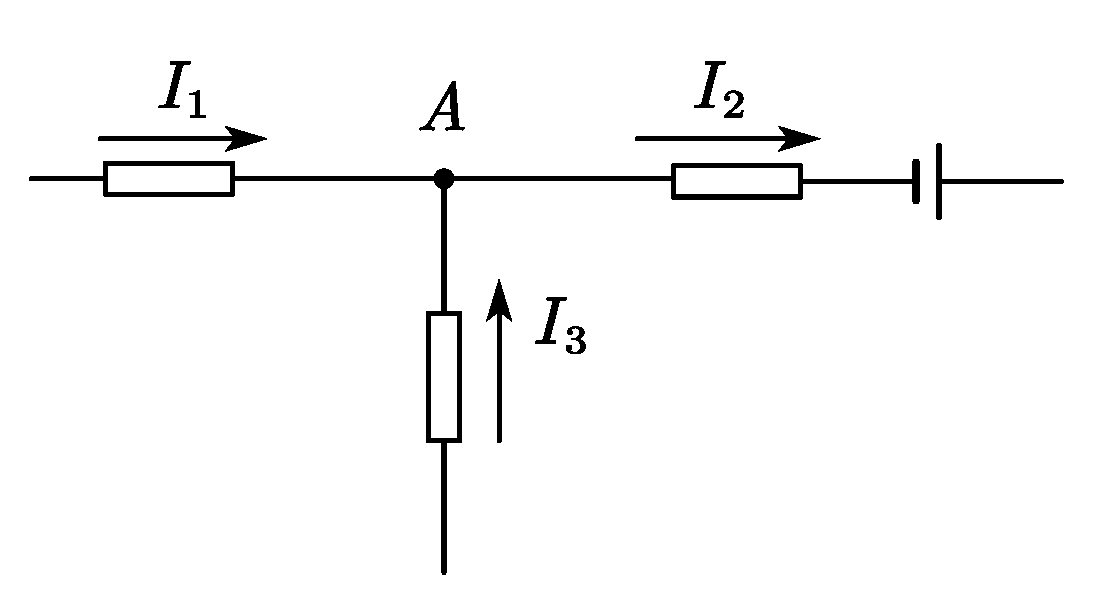
\includegraphics[width=7cm]{./figures/Kirch_1.pdf}
\caption{列节点方程} \label{Kirch_fig1}
\end{figure}
各支路电流往往是未知量,它们的方向事先并不知道.这时,可以先给每个支路电流假设一个方向,并按照这一方向列出方程.求解方程后,如果求得某支路电流的数值为正,则该电流的实际方向与假设方向相同,否则相反.这个假设的电流方向叫做电流的\textbf{正方向}.给每一支路电流假设一个正方向之后,就可用代数量描写每条支路的电流,代数量的绝对值反映电流的大小,代数量的正负则反映电流的实际方向.正方向一经选定,节点方程节点方程的形式(等号左右两边应写哪些电流)就完全确定.例如,为列出\autoref{Kirch_fig1}中节点$A$的方程,可任意地选定与$A $有关的三个支路电流的正方向如图箭头所示,从而写出如下的节点方程:
\begin{equation}
I_1+I_3-I_2=0
\end{equation}
\end{example}
电路中有$n$个节点的时候,一共有$n-1$个节点方程是独立的.这$n-1$个独立方程构成\textbf{基尔霍夫第一方程组}.将它们与基尔霍夫第二方程组联立后,可以根据已知电动势及电阻求得每一支路的电流.

\begin{theorem}{基尔霍夫电压定律}
\textbf{基尔霍夫电压定律}又称为\textbf{基尔霍夫第二定律},表明沿着闭合回路所有元件两端的电势差(电压)的代数和等于零.或者,换句话说,沿着闭合回路的所有电动势的代数和等于所有电压降的代数和.以方程式表达,对于电路的任意闭合回路,
\begin{equation}\label{Kirch_eq1}
\sum_{k=1}^m U_k = 0
\end{equation}
其中,$m$是此闭合回路的元件数目,$U_k$是元件两端的电压,可以是实数或复数.
\end{theorem}

\subsubsection{证明}
根据电势差的定义(\autoref{Voltag_eq1}\upref{Voltag})
\begin{equation}
U_{21} = V(\bvec r_2) - V(\bvec r_1) = - \int_{\bvec r_1}^{\bvec r_2} \bvec E_0(\bvec r) \vdot \dd{\bvec r}
\end{equation}
如果令路径起点为 $\bvec r_1$, 终点为 $\bvec r_N$, 中途有若干点 $\bvec r_2, \dots, \bvec r_{N-1}$. 那么有可以将路径积分划分为若干段, 总电势差等与每段电势差之和
\begin{equation}
U_{N1} = U_{21} + U_{32} + \dots + U_{N, N-1}
\end{equation}
其中 $U_{j, i} = - \int_{\bvec r_i}^{\bvec r_{j}} \bvec E_0(\bvec r) \vdot \dd{\bvec r}$.
如果取一个环路作为积分路径, 起点终点相接, 电势差为零. 即 $\bvec r_1 = \bvec r_N$, $U_{N1} = 0$. 立即可得\autoref{Kirch_eq1}. 证毕.

\begin{example}{}
\begin{figure}[ht]
\centering
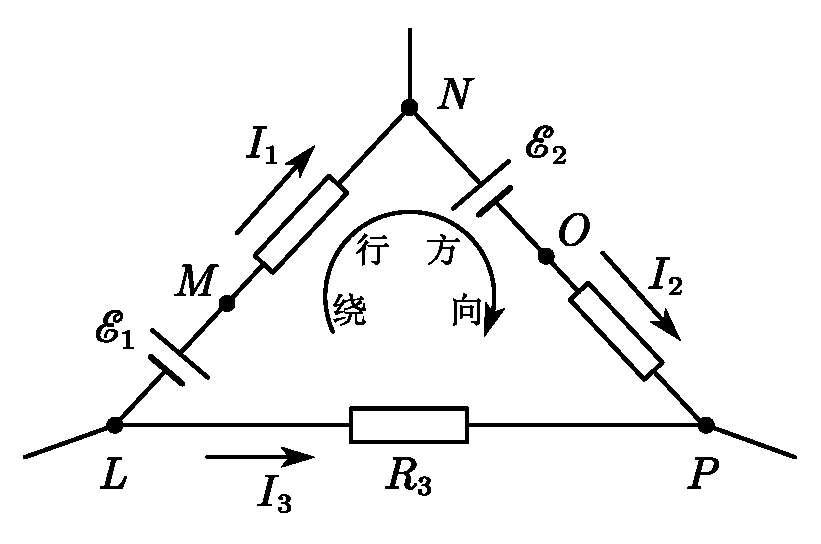
\includegraphics[width=8cm]{./figures/Kirch_2.pdf}
\caption{复杂电路中的一个回路} \label{Kirch_fig2}
\end{figure}

据\autoref{Kirch_fig2},由基尔霍夫电压定律可知,
\begin{equation} \label{Kirch_eq2}
U_{M L}+U_{N M}+U_{O N}+U_{P O}+U_{L P}=0
\end{equation}
设想有一个观察者从$L$点出发沿图中圆形箭头所示的方向绕行回路一周回到$L $点,他沿途看到电势有时升高有时降低,而且升、降的总量相等.由图看出,电势从$L $到$M $升高了数值$\mathscr E_1$,从$M $到$N $降低了数值$I_1R_1$,依次类推,于是\autoref{Kirch_eq2}可以表示为
\begin{equation}\label{Kirch_eq3}
\mathscr{E}_{1}-I_{1} R_{1}-\mathscr{E}_{2}-I_{2} R_{2}+I_{3} R_{3}=0
\end{equation}

由以上讨论不难看\autoref{Kirch_eq3}中每项前面的正、负号应由以下规则确定:任意选定一个绕行回路的方向(叫做绕行方向),当绕行方向从负极进入电源时(如$\mathscr E_1$),其电动势前写$+$号,否则写$-$号(如$\mathscr
E_2$);当绕行方向与电阻的电流正方向相同时(如$R_1$和$R_3$),该电阻的$IR$项前写$-$号, 否则写$+$号(如$R_2$). 再次强调电流可正可负, 正电流表示与正方向形同, 负电流则相反, 所以 $IR$ 也可正可负.
\end{example}

一个电路可以包含许多回路,但它们的方程并非都是独立的.如下图电路所示:$AR_2BR_1A$、$AR_3BR_2A$及$AR_3BR_1A$.
\begin{figure}[ht]
\centering
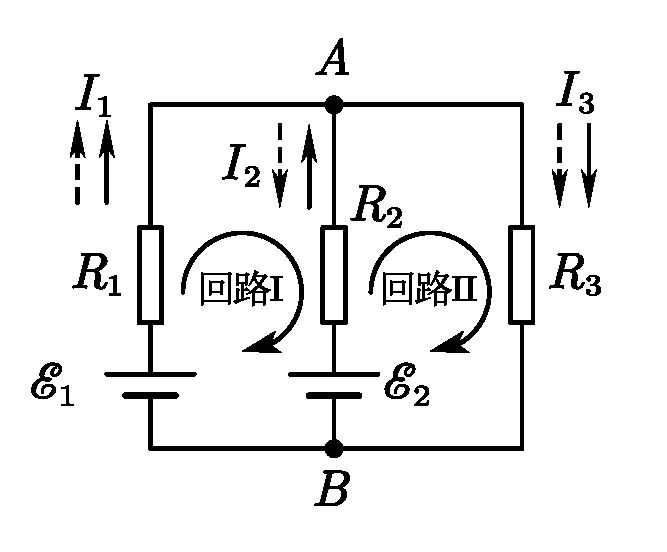
\includegraphics[width=5.5cm]{./figures/Kirch_3.pdf}
\caption{独立回路} \label{Kirch_fig3}
\end{figure}

前两个回路的方程显然独立,因为每个回路都包含一条另一回路所不包含的支路.但第三个回路的方程就不独立,它可由前两个方程推出.电路中所有独立的回路方程构成\textbf{基尔霍夫第二方程组}.为了列出独立的回路方程,可以选择这样的回路,其中每个至少包含一条其他回路所不包含的支路.一个完整电路的支路数$b$、节点数$n $和独立回路数$m $之间的关系为
\begin{equation}
b=m+n-1
\end{equation}

如果全部电动势及电阻皆已知,则电路共有$b $个未知的支路电流.另一方面,由前述可知,这个电路必有$n-1 $个独立的节点方程及$m $个独立的回路方程,即共有$m + n -1$个独立方程,恰与未知量个数$b $相等,因此可唯一地解出各支路电流.当然,除支路电流外,电动势或电阻也可作为未知量,只要未知量个数为$b$,同样可以求解.可见基尔霍夫方程组原则上可以解决一切线性直流电路的计算问题.

当电动势是待求量而且连电源的极性也未知时,可以任意地给电动势选定一个正方向(即假设一对正、负极,电动势的正方向是指从假设的负极到正极的方向),并把电动势作为代数量列出基氏第二方程,方程中$\mathscr E$前的$+$、$-$号应根据绕行方向是否进入假设的负极来决定.求解后,如果$\mathscr E>0$,则实际极性与假设极性相同,否则相反.